In einem anharmonische Oszillator oszilliert eine Masse $m$ unter dem
Einfluss einer Kraft, die nach dem Gesetz
\[
F(x) = -\kappa x + \delta x^3
\]
von der Auslenkung aus der Ruhelage abhängt.
Nehmen Sie im Folgenden an, dass $\delta >0$ ist,
dass also die rücktreibende Kraft $F(x)$ kleiner ist als bei einem
harmonischen Oszillator.
Ziel der folgenden Teilaufgaben ist, die Lösung $x(t)$ schrittweise
dadurch zu bestimmen, dass die Bewegungsgleichung in die Differentialgleichung
der Jacobischen elliptischen Funktion $\operatorname{sn}(u,k)$ umgeformt
wird.
\begin{teilaufgaben}
\item
Berechnen Sie die Auslenkung $x_0$, bei der die rücktreibende Kraft
verschwindet.
Eine beschränkte Schwingung kann diese Amplitude nicht überschreiten.
\item
Berechnen Sie die potentielle Energie in Abhängigkeit von der 
Auslenkung.
\item
\label{buch:1101:basic-dgl}
Formulieren Sie den Energieerhaltungssatz für die Gesamtenergie $E$
dieses Oszillators.
Leiten Sie daraus eine nichtlineare Differentialgleichung erster Ordnung
for den anharmonischen Oszillator ab, die sie in der Form
$\frac12m\dot{x}^2 = f(x)$ schreiben.
\item
Die Amplitude der Schwingung ist derjenige $x$-Wert, für den die
Geschwindigkeit verschwindet.
Leiten Sie die Amplitude aus der Differentialgleichung von
\ref{buch:1101:basic-dgl} ab.
Sie erhalten zwei Werte $x_{\pm}$, wobei der kleinere $x_-$
die Amplitude einer beschränkten Schwingung beschreibt,
während die $x_+$ die minimale Ausgangsamplitude einer gegen
$\infty$ divergenten Lösung ist.
\item
Rechnen Sie nach, dass
\[
\frac{x_+^2+x_-^2}{2}
=
x_0^2
\qquad\text{und}\qquad
x_-^2x_+^2
=
\frac{4E}{\delta}.
\]
\item
Faktorisieren Sie die Funktion $f(x)$ in der Differentialgleichung
von Teilaufgabe c) mit Hilfe der in Teilaufgabe d) bestimmten 
Nullstellen $x_{\pm}^2$.
\item
Dividieren Sie die Differentialgleichung durch $x_-^2$, schreiben
Sie $X=x/x_-$ und bringen Sie die Differentialgleichung in die
Form
\begin{equation}
A \dot{X}^2
=
(1-X^2)
(1-k^2X^2),
\label{buch:1101:eqn:dgl3}
\end{equation}
wobei $k^2=x_-^2/x_+^2$ und $A$ geeignet gewählt werden müssen.
\item
\label{buch:1101:teilaufgabe:dgl3}
Verwenden Sie $t(\tau) = \alpha\tau$
und
$Y(\tau)=X(t(\tau))$ um eine Differentialgleichung für die Funktion
$Y(\tau)$ zu gewinnen, die die Form der Differentialgleichung
von $\operatorname{sn}(u,k)$ hat, für die also $A=0$ in
\eqref{buch:1101:eqn:dgl3} ist.
\item
Verwenden Sie die Lösung $\operatorname{sn}(u,k)$ der in 
\ref{buch:1101:teilaufgabe:dgl3} erhaltenen Differentialgleichung,
um die Lösung $x(t)$ der ursprünglichen Gleichung aufzuschreiben.
\end{teilaufgaben}

\begin{loesung}
\begin{figure}
\centering
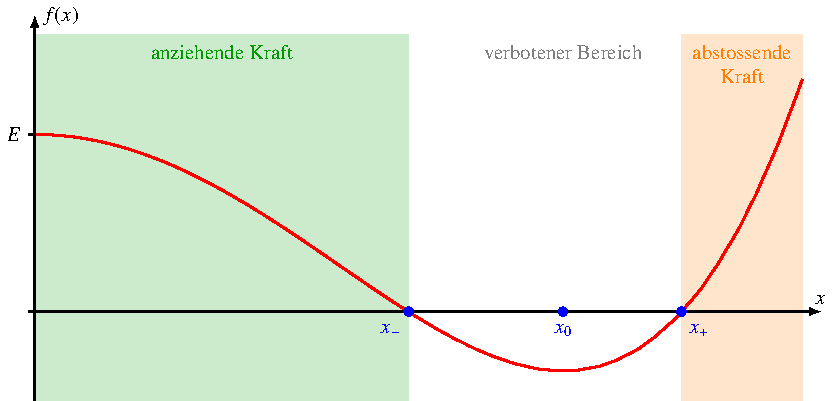
\includegraphics{chapters/110-elliptisch/uebungsaufgaben/anharmonisch.pdf}
\caption{Rechte Seite der Differentialgleichung
\eqref{buch:1101:eqn:dglf}. 
Eine beschränkte Lösung bewegt sich im Bereich $x<x_-$
während im Bereich $x>x_+$ die Kraft abstossend ist und zu einer
divergenten Lösung führt.
\label{buch:1101:fig:potential}
}
\end{figure}
\begin{teilaufgaben}
\item
Wegen
\[
F(x)
=
-\kappa x\biggl(1-\frac{\delta}{\kappa}x^2\biggr)
=
-Ix
\biggl(1-\sqrt{\frac{\delta}{\kappa}}x\biggr)
\biggl(1+\sqrt{\frac{\delta}{\kappa}}x\biggr)
\]
folgt, dass die rücktreibende Kraft bei der Auslenkung  $\pm x_0$ mit
\[
x_0^2
=
\frac{\kappa}{\delta}
\qquad\text{oder}\qquad
x_0 = \sqrt{\frac{\kappa}{\delta}}
\]
verschwindet.
\item
Die potentielle Energie ist die Arbeit, die gegen die rücktreibende Kraft
geleistet wird, um die Auslenkung $x$ zu erreichen.
Sie entsteht durch Integrieren der Kraft über
das Auslenkungsinterval, also
\[
E_{\text{pot}}
=
-
\int_0^x F(\xi) \,d\xi
=
\int_0^x \kappa\xi-\delta\xi^3\,d\xi
=
\biggl[
\kappa\frac{\xi^2}{2}
-
\delta
\frac{\xi^4}{4}
\biggr]_0^x
=
\kappa\frac{x^2}{2}
-
\delta\frac{x^4}{4}.
\]
\item
Die kinetische Energie ist gegeben durch
\[
E_{\text{kin}}
=
\frac12m\dot{x}^2.
\]
Die Gesamtenergie ist damit
\[
E
=
\frac12m\dot{x}^2
+
\kappa
\frac{x^2}{2}
-
\delta
\frac{x^4}{4}.
\]
Die verlangte Umformung ergibt
\begin{align}
\frac12m\dot{x}^2
&=
E
-
\kappa\frac{x^2}{2}
+
\delta\frac{x^4}{4}
\label{buch:1101:eqn:dglf}
\end{align}
als Differentialgleichung für $x$.
Die Ableitung $\dot{x}$ hat positives Vorzeichen wenn die Kraft
abstossend ist und negatives Vorzeichen dort, wo die Kraft anziehend ist.
%
\item
Die Amplitude der Schwingung ist derjenige $x$-Wert, für den
die Geschwindigkeit verschwindet, also eine Lösung der Gleichung
\[
0
=
\frac{2E}{m} -\frac{\kappa}{m}x^2 + \frac{\delta}{2m}x^4.
\]
Der gemeinsame Nenner $m$ spielt offenbar keine Rolle.
Die Gleichung hat die zwei Lösungen
\[
x_{\pm}^2
=
\frac{\kappa \pm \sqrt{\kappa^2-4E\delta}}{\delta}
=
\frac{\kappa}{\delta}
\pm
\sqrt{
\biggl(\frac{\kappa}{\delta}\biggr)^2
-
\frac{4E}{\delta}
}.
\]
Die Situation ist in Abbildung~\ref{buch:1101:fig:potential}
Für $x>x_+$ ist die Kraft abstossend, die Lösung divergiert.
Die Lösung mit dem negativen Zeichen $x_-$ bleibt dagegen beschränkt,
dies ist die Lösung, die wir suchen.

\item
Die beiden Formeln ergeben sich aus den Regeln von Vieta für die
Lösungen einer quadratischen Gleichungg der Form $x^4+px^2+q$.
Die Nullstellen haben den Mittelwert $-p/2$ und das Produkt $q$.

\item
Die rechte Seite der Differentialgleichung lässt sich mit Hilfe
der beiden Nullstellen $x_{\pm}^2$ faktorisieren und bekommt die Form
\[
\frac12m\dot{x}^2
=
\frac{\delta}{4}(x_+^2-x^2)(x_-^2-x^2).
\]

\item
Indem die ganze Gleichung durch $x_-^2$ dividiert wird, entsteht 
\[
\frac12m
\biggl(\frac{\dot{x}}{x_-}\biggr)^2
=
\frac{\delta}{4}
(x_+^2-x^2)
\biggl(1-\frac{x^2}{x_-^2}\biggr).
\]
Schreiben wir $X=x/x_-$ wird daraus
\[
\frac1{2}m\dot{X}^2
=
\frac{\delta}{4}
\biggl(x_+^2-x_-^2 X^2\biggr)
(1-X^2).
\]
Durch Ausklammern von $x_+^2$ im ersten Faktor  wir daraus
\[
\frac1{2}m\dot{X}^2
=
\frac{\delta}{4}
x_+^2
\biggl(1-\frac{x_-^2}{x_+^2} X^2\biggr)
(1-X^2).
\]
Mit der Schreibweise $k^2 = x_-^2/x_+^2$ wird die Differentialgleichung
zu
\begin{equation}
\frac{2m}{\delta x_+^2} \dot{X}^2
=
(1-X^2)(1-k^2X^2),
\label{buch:1101:eqn:dgl2}
\end{equation}
was der Differentialgleichung für die Jacobische elliptische Funktion
$\operatorname{sn}(u,k)$ bereits sehr ähnlich sieht.
\item
Bis auf den Faktor vor $\dot{X}^2$ ist 
\eqref{buch:1101:eqn:dgl2}
die Differentialgleichung
von
$\operatorname{sn}(u,k)$.
Um den Faktor zum Verschwinden zu bringen, schreiben wir 
$t(\tau) = \alpha\tau$.
Die Ableitung von $Y(\tau)=X(t(\tau))$ nach $\tau$ ist
\[
\frac{dY}{d\tau}
=
\dot{X}(t(\tau))\frac{dt}{d\tau}
=
\alpha
\dot{X}(t(\tau))
\qquad\Rightarrow\qquad
\frac{1}{\alpha^2}\frac{dY}{d\tau}
=
\dot{X}(t(\tau)).
\]
Die Differentialgleichung für $Y(\tau)$ ist
\[
\frac{2mk^2}{\delta x_+^2\alpha^2}
\frac{dY}{d\tau}
=
(1-Y^2)(1-k^2Y^2).
\]
Der Koeffizient vor der Ableitung wird $1$, wenn man 
\[
\alpha^2
=
\frac{2mk^2}{\delta x_+^2}
\]
wählt.
Diese Differentialgleichug hat die Lösung
\[
Y(\tau) = \operatorname{sn}(\tau,k).
\]
\item
Indem man die gefunden Grössen einsetzt kann man jetzt die Lösung 
der Differentialgleichung in geschlossener Form als
\begin{align*}
x(t)
&=
x_- X(t)
=
x_- \operatorname{sn}\biggl(
t\sqrt{\frac{\delta x_+^2}{2mk^2} }
,k
\biggr)
\end{align*}
Das Produkt $\delta x_+^2$ kann auch als
\[
\delta x_+^2
=
\kappa+\sqrt{\kappa -4\delta E}
\]
geschrieben werden.
\qedhere
\end{teilaufgaben}
\end{loesung}


